\documentclass[10pt,twocolumn,letterpaper]{article}
\usepackage[top=0.75in,bottom=1in,left=0.625in,right=0.625in,columnsep=0.25in]{geometry}
\usepackage[T1]{fontenc}
\usepackage[utf8]{inputenc}
\usepackage{mathptmx}
\usepackage{amsmath}
\usepackage{graphicx}
\usepackage{booktabs}
\usepackage{xcolor}
\usepackage[hidelinks]{hyperref}
\usepackage{xurl}
\urlstyle{same}
\renewcommand{\ttdefault}{pcr}
\usepackage{cite}
\usepackage{titlesec}
\usepackage[font=footnotesize,labelsep=period]{caption}
\usepackage{enumitem}
\usepackage{balance}
\usepackage{microtype}
% Links shown in the paper. Recompile with: pdflatex paper.tex (twice)
\newcommand{\PROFNAME}{Alexandra de la Cruz Puente}
\newcommand{\PROFMAIL}{alexandra.lacruz@unibague.edu.co}
\newcommand{\GITHUBURL}{https://github.com/rosembergcardona-cmd/rutasIbague}
\newcommand{\DRIVEURL}{https://drive.google.com/drive/folders/1dqNyADbWHi20WrNFY8ZSJ-veMudIHfCv}
\newcommand{\APPURL}{https://rutasibague.vercel.app}

\renewcommand{\thesection}{\Roman{section}}
\renewcommand{\thesubsection}{\Alph{subsection}}
\titleformat{\section}{\centering\normalfont\normalsize\scshape}{\thesection.}{0.5em}{}
\titlespacing*{\section}{0pt}{8pt}{4pt}
\titleformat{\subsection}{\normalfont\normalsize\itshape}{\thesubsection.}{0.5em}{}
\titlespacing*{\subsection}{0pt}{6pt}{3pt}
\captionsetup[table]{name=TABLE,labelformat=simple,labelsep=newline,justification=centering,font={footnotesize,sc}}
\renewcommand{\thetable}{\Roman{table}}
\captionsetup[figure]{name=Fig.}
\setlength{\parindent}{1em}
\setlist{nosep,leftmargin=1.2em}
\pagestyle{plain}
\begin{document}
\twocolumn[
\begin{center}
{\LARGE RutaIbagué: A Utility-Based A* Search Agent\\[2pt] for Bus Trip Recommendation in Ibagué, Colombia\par}
\vspace{10pt}
\begin{tabular}{c@{\hspace{3em}}c}
Rosemberg Cardona & \PROFNAME \\
\footnotesize\itshape Universidad de Ibagué & \footnotesize\itshape Universidad de Ibagué \\
\footnotesize\itshape Ibagué, Tolima, Colombia & \footnotesize\itshape Ibagué, Tolima, Colombia \\
\footnotesize rosemberg.cardona@estudiantesunibague.edu.co & \footnotesize \PROFMAIL \\
\end{tabular}
\vspace{12pt}
\end{center}
]

\noindent\textbf{\textit{Abstract}---Collective buses carry about a third of daily trips in Ibagué, Colombia, but riders have little information about which route serves their trip, and no open data on the routes is available. This paper presents RutaIbagué, an intelligent agent that recommends which bus or combination of buses to take. The agent perceives the origin, the destination, the departure time and a user preference; models the network, stored in the GTFS format, as a state graph of stops and route patterns; and uses A* search with an admissible heuristic to find the trip with the lowest generalized cost (walking, waiting, riding and a transfer penalty weighted by the preference). It reports the arrival time with an uncertainty range and abstains when no stop is close enough. The agent is deployed as an installable web application. Because no official data exist, it was evaluated on a pilot network of 8 illustrative routes and 28 stops. Over all 756 stop pairs, A* matched the optimal cost of Dijkstra's algorithm in 100\,\% of the queries while expanding 36.7--44.4\,\% fewer states, and answered in under 0.3\,ms at the 95th percentile. Only 44.4\,\% of the pairs are served by a single direct route, whereas the agent found a trip for all of them. These results validate the agent's design; real route data and field calibration are needed to assess real-world accuracy.}

\vspace{4pt}
\noindent\textbf{\textit{Index Terms}---intelligent agent, A* search, heuristic search, public transport, journey planning, GTFS, utility.}

\section{Introduction}
Ibagué, the capital of Tolima, had 541,101 inhabitants in 2018, 92.7\,\% of them in the urban area. Seven companies operated 30 collective bus routes covering about 90\,\% of the urban perimeter, and buses carried about 34.4\,\% of daily trips, with 74.8 million passengers in 2019 \cite{conpes4017}. The city is implementing a Strategic Public Transport System (SETP), a reform that has caused conflict with operators \cite{bluradio2023}; similar reforms in intermediate Colombian cities have been followed by lower ridership \cite{gomezlobo2020}. In March 2026 the city started a pilot of mandatory bus stops on Carrera Quinta, from Calle 10 to Calle 80 \cite{rcn2026}.

Riders, however, have little support for planning a trip. We found no open dataset of the routes, so a person who does not already know the network cannot easily tell which bus to take, especially when the trip needs a transfer. Our initial proposal was an agent for operators that would predict passenger demand and arrival times. It was narrowed because the required GPS and fare-collection data are not public. The resulting system, RutaIbagué, solves one problem that can be addressed with data that can be collected: \emph{recommending which bus or buses to take}.

The contributions are: (i) a utility-based agent that formulates trip recommendation as an A* search over a stop--route state graph, with an admissible heuristic, a time-of-day context model, an uncertainty range and an abstention rule (Section~\ref{sec:methods}); (ii) a pilot network for Ibagué in the standard GTFS format, so that real data can replace it without code changes; (iii) an installable web application whose code is public \cite{repo}; and (iv) an evaluation of optimality, efficiency, coverage and preference trade-offs (Section~\ref{sec:results}). Section~\ref{sec:related} reviews related work and Section~\ref{sec:conclusions} concludes.

\section{Related Work}\label{sec:related}
\subsection{Data-driven prediction for bus transit}
Passenger-flow forecasting has moved from ARIMA and classical machine learning to deep spatio-temporal models, but most studies concern rail systems and open bus data are scarce \cite{hecht2025}. Graph attention networks predict short-term bus origin--destination demand \cite{cao2025}, neural networks predict bus journey times from GPS \cite{lim2024}, and multi-agent reinforcement learning controls bus bunching in simulation \cite{wang2020}. For small cities with little data, simple direct-demand models are often adequate \cite{shellhamer2019}. All of these require operator data that are not available in Ibagué, which motivated the change of scope described above.

\subsection{Search-based route planning}
Finding a minimum-cost path in a graph with non-negative costs is solved by Dijkstra's algorithm \cite{dijkstra1959}. A* adds a heuristic estimate of the remaining cost; when the heuristic is admissible it still returns an optimal path while usually expanding fewer nodes \cite{hart1968,russell2020}. Route planning in transportation networks is a mature field with speed-up techniques for continental road networks and large timetabled transit networks \cite{bast2016}. RAPTOR works on timetables in rounds, one per transfer, and its multi-criteria variant returns Pareto sets of trips \cite{delling2015}. For a city network with tens of routes, a plain A* over a stop--route state graph is fast enough and easier to explain, which matters in an academic setting.

\subsection{Journey planners and transit data}
Open-source planners such as OpenTripPlanner \cite{otp} combine street and transit networks described in GTFS, the de facto standard for schedules, routes and stops \cite{gtfs}. Where no GTFS feed exists, data can be collected: in Bogotá's Mapatón (2017), university students rode informal bus routes with GPS phone apps and produced a GTFS feed later used by the transit authority \cite{mapaton}. OpenStreetMap provides a guide for mapping public transport in Colombia \cite{osmguide} and a geocoder, Nominatim \cite{nominatim}.

\subsection{Gap}
We found no documented trip planner and no open dataset for Ibagué's collective buses. A small, explainable agent that reads GTFS and can run on collected data addresses a local need and fits the scope of a course project.

\section{Methods}\label{sec:methods}
\subsection{Agent design}
RutaIbagué is a model-based, utility-based problem-solving agent \cite{russell2020}. Fig.~\ref{fig:arch} shows its cycle and Table~\ref{tab:peas} its PEAS description. The knowledge base is the GTFS feed plus a speed model; perception turns the request into a start state, a goal and a context; A* search finds the best trip; the decision step applies the utility and the abstention rule; the action is the trip plan shown to the user.

\begin{figure}[t]
\centering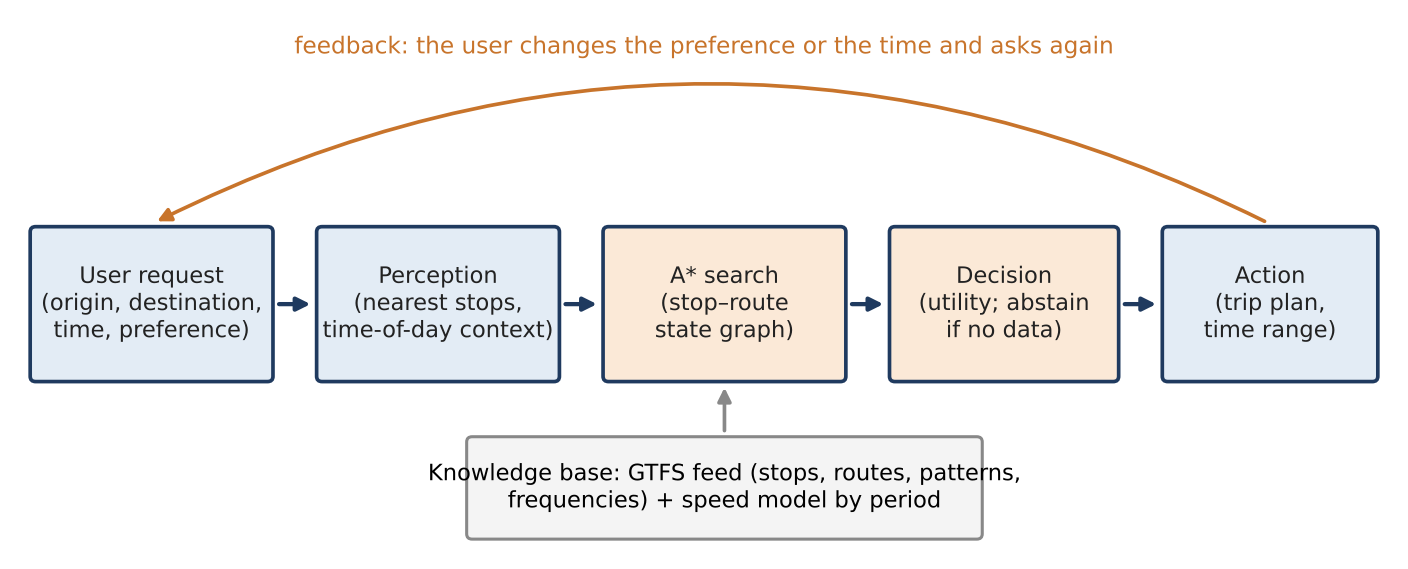
\includegraphics[width=\columnwidth]{../figures/fig1_architecture.png}
\caption{Architecture and perception--decision--action cycle of the agent.}
\label{fig:arch}
\end{figure}

\begin{table}[t]
\caption{PEAS description of the agent}\label{tab:peas}
\centering\footnotesize
\begin{tabular}{@{}p{1.6cm}p{6.3cm}@{}}
\toprule
Performance & Optimal (lowest-cost) trip; total time; transfers; walking; correct abstention; response time \\
Environment & Bus network of Ibagué (pilot: 8 routes, 28 stops) and time of day \\
Actuators & Trip plan, map, arrival time and range, alternatives, abstention message \\
Sensors & Origin and destination (stop, address, GPS location or map point), departure time, preference; GTFS knowledge base \\
\bottomrule
\end{tabular}
\end{table}

\subsection{Dataset}
No open data on Ibagué's routes was found, so we built a pilot network (Fig.~\ref{fig:net}). It has 28 stops at approximate coordinates of well-known places (the city centre, the bus terminal, both universities, shopping centres, the airport and outer districts) and 8 illustrative routes that connect them, with headways between 8 and 20 minutes. \textbf{It is sample data, not the official routes.} The network is stored as a GTFS feed \cite{gtfs} (Table~\ref{tab:gtfs}) with one trip pattern per route and direction, off-peak running times in \texttt{stop\_times.txt}, and headways in \texttt{frequencies.txt} (daytime, 05:00--21:00; double headway at night, 21:00--24:00). The feed and its documentation are in the repository \cite{repo} and on Google Drive \cite{drive}.

\begin{figure}[t]
\centering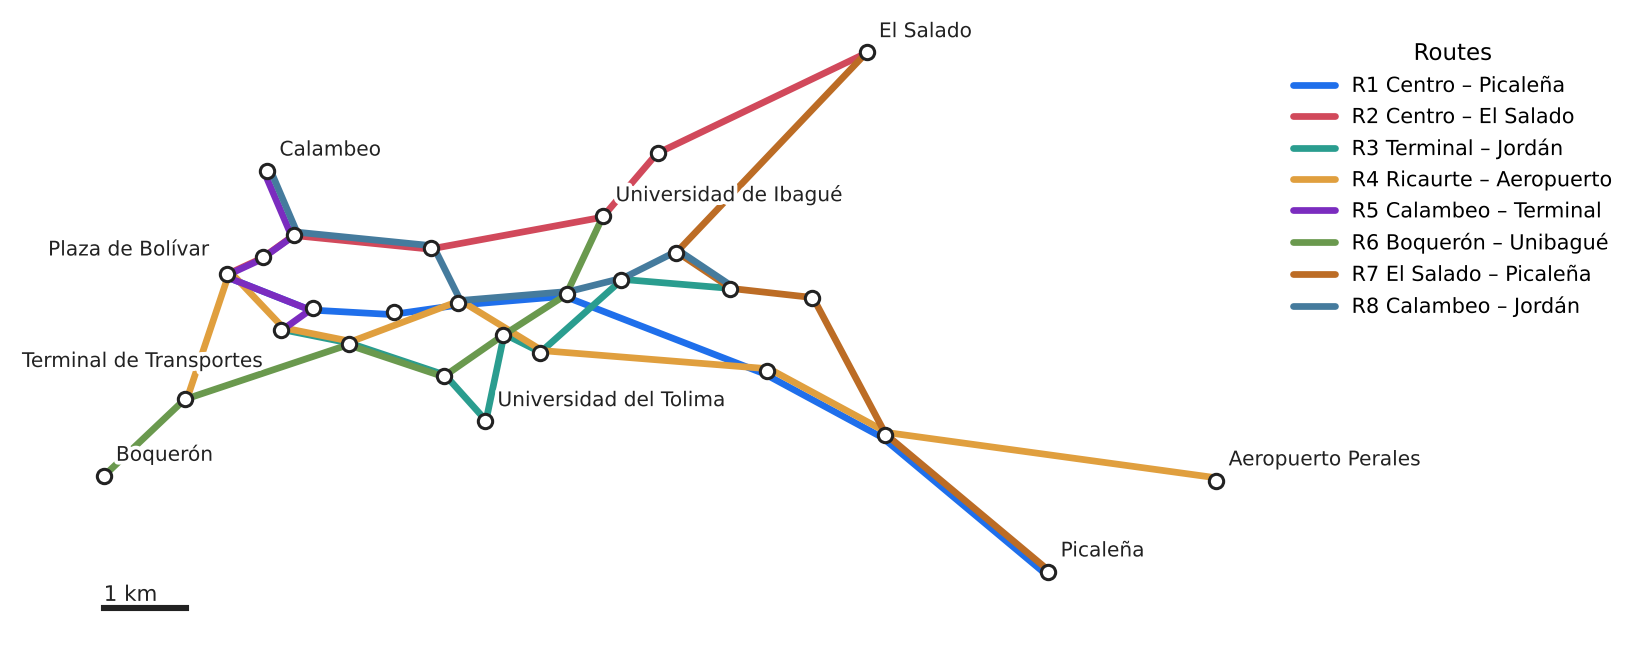
\includegraphics[width=\columnwidth]{../figures/fig2_network.png}
\caption{Pilot network used in this work (sample data; positions are approximate).}
\label{fig:net}
\end{figure}

\begin{table}[t]
\caption{Files of the pilot GTFS feed}\label{tab:gtfs}
\centering\footnotesize
\begin{tabular}{@{}lrl@{}}
\toprule
File & Rows & Content \\
\midrule
stops.txt & 28 & Stop id, name, latitude, longitude \\
routes.txt & 8 & Route id, name, colour \\
trips.txt & 16 & One pattern per route and direction \\
stop\_times.txt & 118 & Stop order and off-peak times \\
frequencies.txt & 32 & Day and night headways \\
\bottomrule
\end{tabular}
\end{table}

\subsection{State space}
The states are: the origin $O$; the destination $D$; ``at stop $s$'' before the first boarding or after alighting; and ``on pattern $p$ at its $i$-th stop''. The actions and their costs (minutes) are:
\begin{itemize}
\item \emph{walk} from $O$ to any stop within 800\,m, between stops within 350\,m (transfers), or to $D$: distance $\times$ 1.25 detour $\div$ 4.5\,km/h;
\item \emph{board} pattern $p$: expected wait of half its headway at that hour, plus a transfer penalty $k$ if it is not the first boarding;
\item \emph{ride} to the next stop: distance $\times$ 1.35 detour $\div$ bus speed, plus 0.4\,min dwell;
\item \emph{alight} at the current stop (cost 0).
\end{itemize}
Patterns are directional, so loop routes with different paths in each direction are represented without changes.

\subsection{A* search and heuristic}
A* expands the state $n$ with the lowest $f(n) = g(n) + h(n)$, where $g(n)$ is the cost so far and
\begin{equation}
h(n) = \frac{d(n, D)}{v_{\max}},
\end{equation}
with $d$ the great-circle distance and $v_{\max}$ the maximum of the bus and walking speeds. Every path from $n$ to $D$ is at least $d(n,D)$ long and no mode moves faster than $v_{\max}$; waits, dwell times and penalties are non-negative. Hence $h$ never overestimates the remaining cost, it is admissible, and A* returns an optimal trip \cite{hart1968}. Running the same code with $h=0$ gives Dijkstra's algorithm, used as a baseline. A binary heap holds the frontier.

\subsection{Utility and preferences}
The search minimizes the generalized cost
\begin{equation}
C = w \cdot T_{\text{walk}} + T_{\text{wait}} + T_{\text{ride}} + k \cdot N_{\text{transfers}},
\end{equation}
whose weights encode the user's preference (Table~\ref{tab:util}). The time shown to the user is the estimated time, not $C$. Raising $k$ cannot increase the number of transfers of the optimal trip, and raising $w$ cannot increase its walking distance; both properties are checked by unit tests.

\begin{table}[t]
\caption{Utility weights by preference}\label{tab:util}
\centering\footnotesize
\begin{tabular}{@{}lcc@{}}
\toprule
Preference & Transfer penalty $k$ & Walking weight $w$ \\
\midrule
Fastest & 3 min & 1.0 \\
Fewest transfers & 12 min & 1.0 \\
Least walking & 3 min & 2.5 \\
\bottomrule
\end{tabular}
\end{table}

\subsection{Context, uncertainty and abstention}
The agent perceives the period of the day from the departure time: peak (6:00--8:30, 11:30--14:00, 17:00--19:30) with an assumed bus speed of 13\,km/h, off-peak with 19\,km/h, and night (from 21:00) with 22\,km/h and the night headways of the feed. These speeds are assumptions to be calibrated with measured trips. The agent reports a time range that widens with riding and waiting time (variability of 20\,\% off-peak, 25\,\% at night and 35\,\% at peak). It recommends walking when the destination is closer than 450\,m and abstains when no stop is within 800\,m of the origin or the destination, or when there is no service at that hour.

\subsection{Implementation}
The application (Fig.~\ref{fig:app}) is a static web page in HTML, CSS and JavaScript with no framework. The agent (\texttt{agent.js}) and the GTFS reader (\texttt{gtfs.js}) run unchanged in the browser and in Node.js. The map is an SVG layer in Web Mercator over OpenStreetMap tiles, with pan, zoom and pinch. Addresses are geocoded with Nominatim \cite{nominatim}, restricted to Ibagué; the user can also type a stop name, use the phone's location or tap the map. The page shows step-by-step instructions, the arrival time and its range, the three preferences side by side, a route catalogue, a link to share the trip and an agent trace (perceived context and states expanded by A* and Dijkstra). A service worker makes it an installable web app that works offline, without tiles and geocoding. The code is versioned on GitHub \cite{repo} and deployed on Vercel at \url{\APPURL}. Node.js runs the unit tests (\texttt{node:test}) and the experiments, and Python with Matplotlib produces the figures.

\begin{figure*}[t]
\centering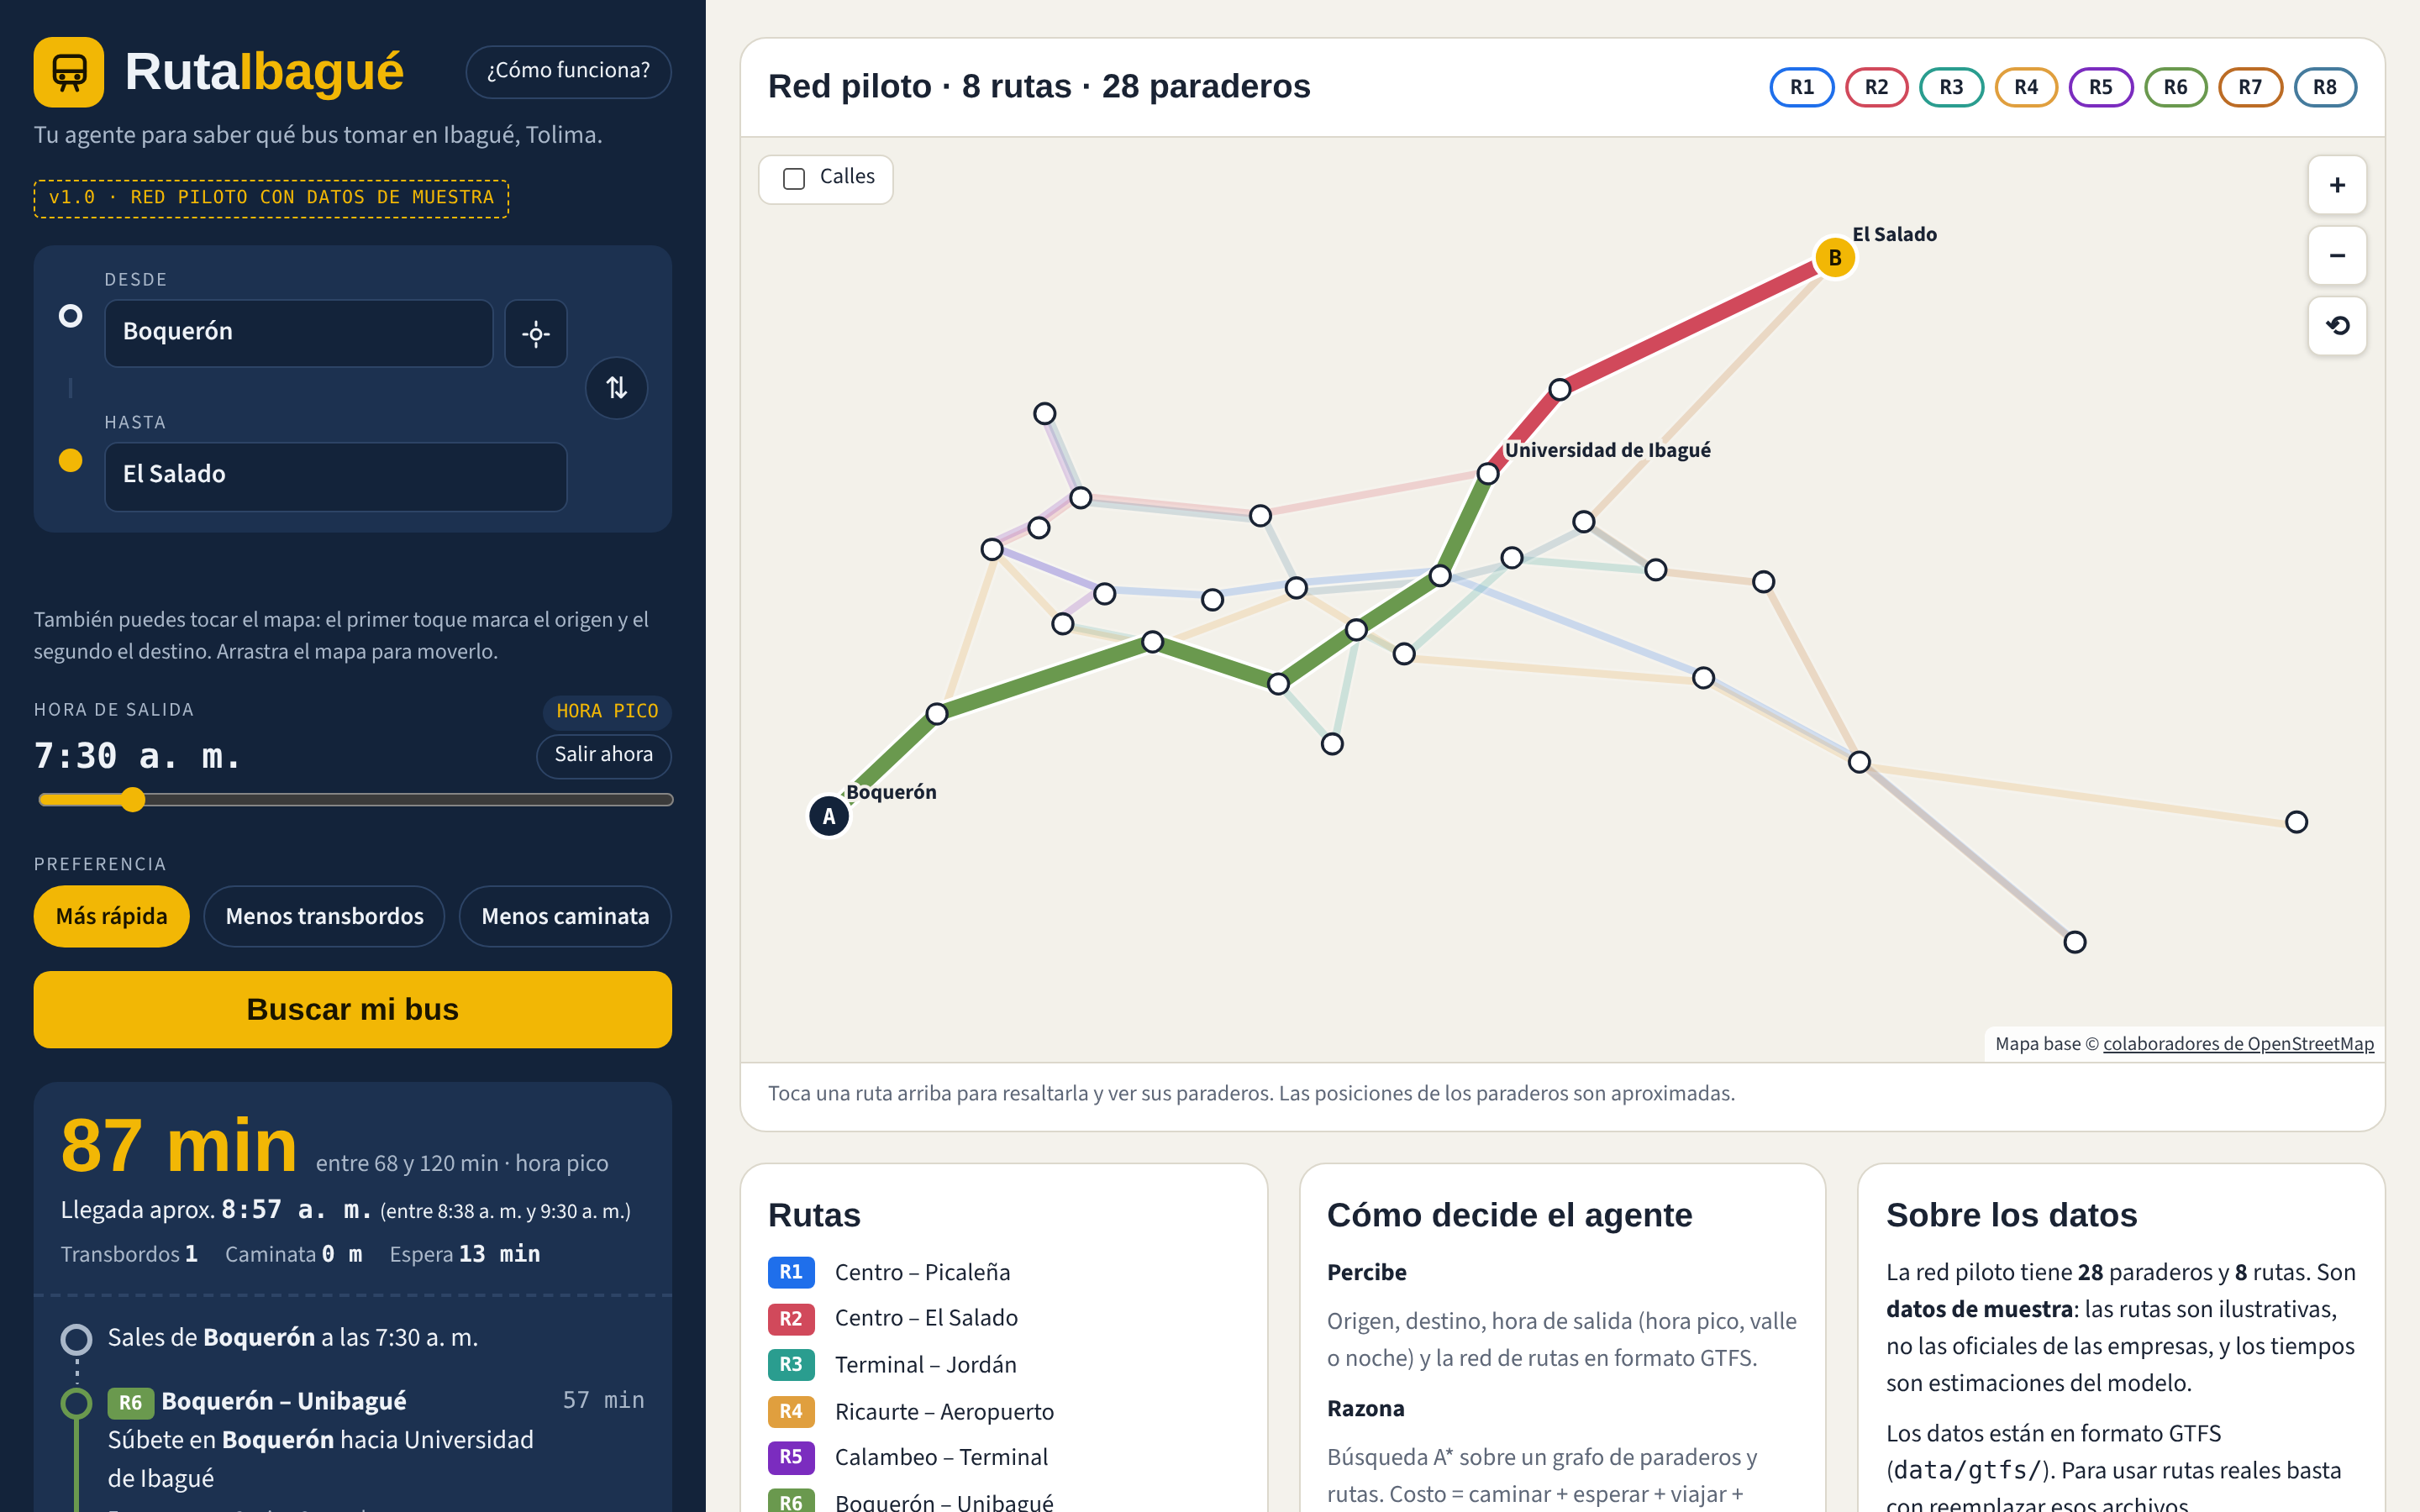
\includegraphics[width=0.86\textwidth]{../figures/fig3_app.png}
\caption{RutaIbagué web application (Spanish interface; street basemap turned off). Trip from Boquerón to El Salado at 7:30 a.m. (peak).}
\label{fig:app}
\end{figure*}

\subsection{Evaluation protocol}
Since no real trips are available for comparison, the evaluation measures the behaviour of the agent on the pilot network:
\begin{itemize}
\item \textbf{E1 Optimality and efficiency.} All 756 ordered stop pairs, solved with A* and Dijkstra at 7:00 (peak), 15:00 (off-peak) and 22:00 (night).
\item \textbf{E2 Coverage.} Share of pairs served by a single direct pattern, a baseline for a rider who only knows individual routes, versus the agent.
\item \textbf{E3 Decisions and preferences.} 500 synthetic trips with origins and destinations placed up to 1.2\,km from random stops (seeded), off-peak.
\item \textbf{E4 Time of day.} Mean trip time, wait and range width per period over all pairs.
\end{itemize}
Eleven unit tests check the GTFS loading, the context, the optimality of A*, the admissibility of the heuristic, the monotonicity of the preferences, abstention, the walking rule, service hours, the time range and the order of bus legs. All pass.

\section{Results}\label{sec:results}
\subsection{Optimality and efficiency of A*}
A* returned the same optimal cost as Dijkstra in 100\,\% of the 2,268 queries (Table~\ref{tab:e1}). It expanded 44.4\,\% fewer states at peak, 41.9\,\% off-peak and 36.7\,\% at night (Fig.~\ref{fig:states}). The reduction is largest at peak because the heuristic is tighter when the bus speed is low. Mean query time with A* was below 0.1\,ms, with a 95th percentile of at most 0.26\,ms in Node.js on a cloud Linux container, so the agent answers instantly in the browser.

\begin{table}[t]
\caption{A* versus Dijkstra on 756 stop pairs per period}\label{tab:e1}
\centering\footnotesize
\begin{tabular}{@{}lccccc@{}}
\toprule
Period & Same cost & States A* & States Dijkstra & Reduction & p95 (ms) \\
\midrule
Peak & 100\,\% & 36.6 & 65.7 & 44.4\,\% & 0.26 \\
Off-peak & 100\,\% & 36.9 & 63.5 & 41.9\,\% & 0.19 \\
Night & 100\,\% & 33.8 & 53.4 & 36.7\,\% & 0.19 \\
\bottomrule
\end{tabular}
\end{table}

\begin{figure}[t]
\centering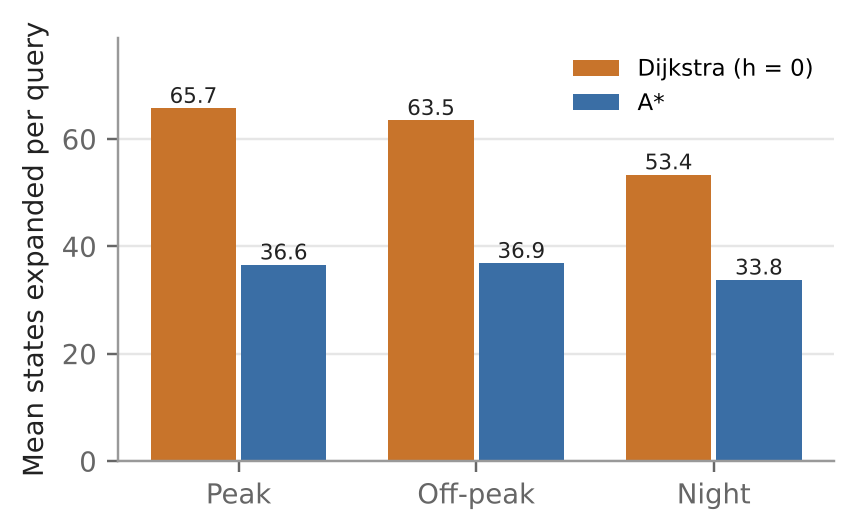
\includegraphics[width=0.9\columnwidth]{../figures/fig4_states.png}
\caption{Mean states expanded per query by A* and Dijkstra.}
\label{fig:states}
\end{figure}

\subsection{Coverage against a direct-route baseline}
Only 44.4\,\% of the stop pairs are served by a single direct pattern; the agent found a trip for 100\,\% of them by combining routes. Of all agent trips, 65.6\,\% need no transfer, 30.2\,\% one, 4.0\,\% two and 0.3\,\% three. When a direct route exists, the agent was faster in only 7.1\,\% of the pairs (mean gain 0.2\,min, maximum 8.8\,min). The main benefit of the agent is therefore enabling trips that need a transfer, not speeding up direct ones.

\subsection{Decisions and preference trade-offs}
Of the 500 synthetic trips, the agent recommended a bus in 54.6\,\%, walking in 18.6\,\% and abstained in 26.8\,\%, because the pilot network does not cover those points. Fig.~\ref{fig:pref} shows the effect of the preference on the 273 bus trips: \emph{fewest transfers} reduced transfers by 34\,\% (0.32 to 0.21 per trip) at the cost of 21\,\% more walking and 0.8\,min more; \emph{least walking} reduced walking by 9\,\% (803 to 731\,m) at the cost of more transfers. The utility therefore produces the intended trade-offs.

\begin{figure}[t]
\centering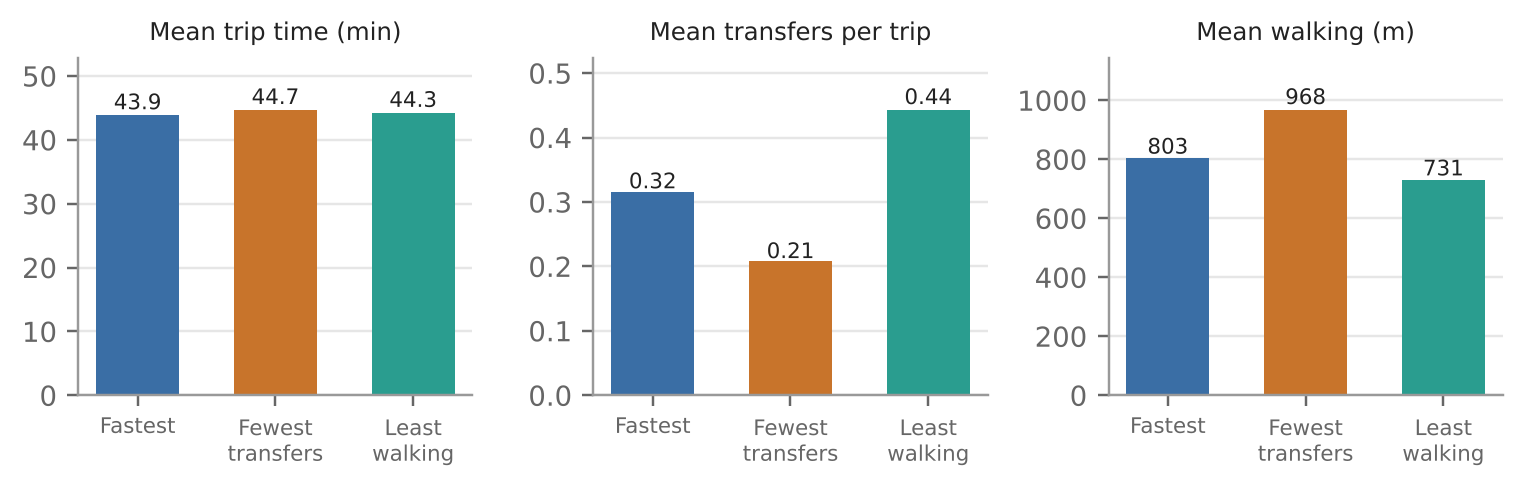
\includegraphics[width=\columnwidth]{../figures/fig5_preferences.png}
\caption{Effect of the user preference on 273 bus trips (off-peak).}
\label{fig:pref}
\end{figure}

\subsection{Effect of the time of day}
Table~\ref{tab:e4} shows that the context model changes the recommendation as intended: the mean trip takes 41.4\,min at peak and 32.6\,min off-peak, and the range shown to the user is wider at peak (23.9\,min) than off-peak (15.5\,min). At night trips are faster than at peak but waits are longer (13.2\,min) because of the lower frequency.

\begin{table}[t]
\caption{Mean values over all stop pairs by period}\label{tab:e4}
\centering\footnotesize
\begin{tabular}{@{}lccc@{}}
\toprule
Period & Trip time (min) & Wait (min) & Range width (min) \\
\midrule
Peak & 41.4 & 8.1 & 23.9 \\
Off-peak & 32.6 & 8.5 & 15.5 \\
Night & 37.9 & 13.2 & 21.0 \\
\bottomrule
\end{tabular}
\end{table}

\subsection{Limitations}
All results describe the agent on a sample network. They do not measure accuracy against real trips: stop positions, routes, speeds and headways are approximate or assumed. The speed model uses three fixed periods, waits assume random arrivals at the stop, and real-time bus positions are not used.

\section{Conclusions}\label{sec:conclusions}
RutaIbagué shows that a classical, explainable AI technique can address a real mobility need in Ibagué with data that can be collected. The agent combines context perception, informed A* search with an admissible heuristic, a utility that encodes user preferences, an uncertainty range and abstention. On the pilot network, A* was always optimal, expanded up to 44\,\% fewer states than Dijkstra, and connected all stop pairs, against 44\,\% with direct routes only. The preferences produced the expected trade-offs. Because the network is stored in GTFS, the next steps require no changes to the code: (1) map the real routes and stops by riding them with a GPS logger, following the Mapatón approach \cite{mapaton,osmguide}; (2) calibrate the speeds and headways by period with measured trips, for example with a regression model; (3) validate the estimated times and ranges against those trips; and (4) test the application with riders.

\section{Code, Data and Video Availability}\label{sec:avail}
\noindent Web application: \url{\APPURL}. The source code, the tests and the experiments are in the GitHub repository \cite{repo}: \url{\GITHUBURL}. The dataset (GTFS feed and experiment results) and the promotional video are in a Google Drive folder \cite{drive}: \url{\DRIVEURL}.

\balance
\footnotesize
\begin{thebibliography}{99}
\bibitem{conpes4017} Consejo Nacional de Política Económica y Social, ``Declaración de importancia estratégica del proyecto Sistema Estratégico de Transporte Público (SETP) de Ibagué,'' Documento CONPES 4017, Departamento Nacional de Planeación, Bogotá, Colombia, Dec. 2020.
\bibitem{bluradio2023} ``Ibagué tiene que modernizar su flota: alcalde responde a paro de transportadores,'' \emph{Blu Radio}, Jul. 26, 2023. [Online]. Available: \url{https://www.bluradio.com/nacion/ibague-tiene-que-modernizar-su-flota-alcalde-responde-a-paro-de-transportadores-so35}
\bibitem{gomezlobo2020} A. Gómez-Lobo, ``Transit reforms in intermediate cities of Colombia: An ex-post evaluation,'' \emph{Transp. Res. A, Policy Pract.}, vol. 132, pp. 349--364, 2020.
\bibitem{rcn2026} ``Ibagué arranca plan piloto para uso obligatorio de paraderos de bus: ¿Dónde aplica?,'' \emph{RCN Radio}, Mar. 2, 2026. [Online]. Available: \url{https://newsroom.rcnradio.com/colombia/ibague-arranca-plan-piloto-para-uso-obligatorio-de-paraderos-de-bus-donde-aplica}
\bibitem{repo} R. Cardona, ``RutaIbagué: source code, data and experiments,'' GitHub repository, 2026. [Online]. Available: \url{\GITHUBURL}
\bibitem{hecht2025} J. Hecht, W. Li, Z. Li, and Y. Dehbi, ``Review of passenger flow modelling approaches based on a bibliometric analysis,'' arXiv:2511.13742, 2025.
\bibitem{cao2025} Z. Cao, L. Song, S. Zhang, and J. Sun, ``Deep learning-driven bus short-term OD demand prediction via a physics-guided adaptive graph spatio-temporal attention network,'' \emph{Sensors}, vol. 25, no. 21, Art. no. 6739, 2025.
\bibitem{lim2024} Y. T. Lim, S. L. Keoh, Y.-W. Chong, N. F. Ibrahim, and A. R. Sharul Kamal, ``An ANN-based prediction model for public bus journey time,'' in \emph{Proc. 6th Int. Conf. Artif. Intell. Inf. Commun. (ICAIIC)}, Osaka, Japan, 2024, pp. 578--583.
\bibitem{wang2020} J. Wang and L. Sun, ``Dynamic holding control to avoid bus bunching: A multi-agent deep reinforcement learning framework,'' \emph{Transp. Res. C, Emerg. Technol.}, vol. 116, Art. no. 102661, 2020.
\bibitem{shellhamer2019} N. J. Shellhamer, ``Direct demand estimation for bus transit in small cities,'' M.S. thesis, Purdue Univ., West Lafayette, IN, USA, 2019.
\bibitem{dijkstra1959} E. W. Dijkstra, ``A note on two problems in connexion with graphs,'' \emph{Numerische Mathematik}, vol. 1, pp. 269--271, 1959.
\bibitem{hart1968} P. E. Hart, N. J. Nilsson, and B. Raphael, ``A formal basis for the heuristic determination of minimum cost paths,'' \emph{IEEE Trans. Syst. Sci. Cybern.}, vol. 4, no. 2, pp. 100--107, Jul. 1968.
\bibitem{russell2020} S. Russell and P. Norvig, \emph{Artificial Intelligence: A Modern Approach}, 4th ed. Hoboken, NJ, USA: Pearson, 2020.
\bibitem{bast2016} H. Bast \emph{et al.}, ``Route planning in transportation networks,'' in \emph{Algorithm Engineering}, LNCS vol. 9220. Cham, Switzerland: Springer, 2016, pp. 19--80.
\bibitem{delling2015} D. Delling, T. Pajor, and R. F. Werneck, ``Round-based public transit routing,'' \emph{Transp. Sci.}, vol. 49, no. 3, pp. 591--604, 2015.
\bibitem{otp} OpenTripPlanner, ``OpenTripPlanner: Multimodal trip planning software.'' [Online]. Available: \url{https://www.opentripplanner.org/}
\bibitem{gtfs} MobilityData, ``General Transit Feed Specification (GTFS).'' [Online]. Available: \url{https://gtfs.org/}
\bibitem{mapaton} ``Fixing the system without breaking it: What cities can learn from Bogotá's Mapatón,'' \emph{Atlas of Popular Transport}, Massachusetts Institute of Technology. [Online]. Available: \url{https://atlasofpopulartransport.mit.edu/bogota}
\bibitem{osmguide} OpenStreetMap Wiki, ``Colombia/Guide for mapping/public transport.'' [Online]. Available: \url{https://wiki.openstreetmap.org/wiki/Colombia/Guide_for_mapping/public_transport}
\bibitem{nominatim} Nominatim, ``Open-source geocoding with OpenStreetMap data.'' [Online]. Available: \url{https://nominatim.org/}
\bibitem{drive} R. Cardona, ``RutaIbagué: dataset and promotional video,'' Google Drive folder, 2026. [Online]. Available: \url{\DRIVEURL}
\end{thebibliography}
\end{document}
